% Presentazione - Cartella clinica passwordless
% Compilare con pdfLaTeX. Le figure sono nella cartella figure/.
\documentclass[11pt,aspectratio=169]{beamer}
\usepackage[utf8]{inputenc}
\usepackage[T1]{fontenc}
\usepackage[italian]{babel}
\usepackage{lmodern}
\usepackage{booktabs}
\usepackage{tikz}
\usetikzlibrary{positioning,arrows.meta,fit}

\usetheme[progressbar=frametitle,numbering=fraction]{metropolis}
\definecolor{accent}{HTML}{17695D}
\definecolor{scuro}{HTML}{23373B}
\definecolor{chiaro}{HTML}{E8F1EF}
\setbeamercolor{frametitle}{bg=scuro,fg=white}
\setbeamercolor{progress bar}{fg=accent,bg=chiaro}
\setbeamercolor{alerted text}{fg=accent}
\setbeamercolor{title separator}{fg=accent}
\setbeamertemplate{itemize item}{\color{accent}\raisebox{.15ex}{$\blacktriangleright$}}

\tikzset{
  box/.style={draw=accent,fill=chiaro,rounded corners=3pt,align=center,font=\small,minimum height=1.1cm,text width=2.1cm},
  freccia/.style={-{Latex[length=2mm]},thick,draw=scuro},
  etichetta/.style={font=\scriptsize,fill=white,inner sep=1.5pt}
}

\title{Cartella clinica passwordless}
\subtitle{Consenso, accesso e audit con FIDO2 e blockchain}
\author{Raffaele}
\institute{Laurea magistrale in Informatica, curriculum Sicurezza Informatica\\Università degli Studi di Salerno}
\date{Sicurezza dei Dati \,---\, A.A. 2026/27}

\begin{document}

\maketitle

% ---------------------------------------------------------------
\begin{frame}{Il problema}
I dati sanitari sono una \alert{categoria particolare} di dati personali (art.~9 GDPR): una fuga causa danni difficili da rimediare.

\bigskip
Nelle cartelle cliniche elettroniche di oggi:
\begin{itemize}
  \item l'accesso si basa su \alert{password}, esposte a phishing e riuso;
  \item il \alert{consenso} del paziente è un documento che il sistema non verifica a ogni accesso;
  \item il \alert{registro degli accessi} è gestito da chi dovrebbe essere controllato.
\end{itemize}
\end{frame}

% ---------------------------------------------------------------
\begin{frame}{Obiettivi}
\begin{columns}[T]
\column{.5\textwidth}
\begin{block}{Accesso senza password}
Passkey FIDO2: resistente a phishing e replay, nessun segreto sul server.
\end{block}
\begin{block}{Consenso verificabile}
Il paziente lo concede e lo revoca dal proprio wallet, per finalità e con scadenza.
\end{block}
\column{.5\textwidth}
\begin{block}{Audit non modificabile}
Ogni accesso, concesso o negato, è scritto su blockchain \emph{prima} della consegna dei dati.
\end{block}
\begin{block}{Dati esposti al minimo}
Sulla catena solo pseudonimi e impronte; referti cifrati fuori dalla catena.
\end{block}
\end{columns}
\end{frame}

% ---------------------------------------------------------------
\begin{frame}{Modello di minaccia}
\begin{tabular}{@{}p{.42\textwidth}p{.52\textwidth}@{}}
\toprule
Minaccia & Difesa\\
\midrule
Phishing, replay delle credenziali & Firma legata all'origin, challenge monouso\\
Autenticatore clonato & Contatore anti-riuso con compare-and-set\\
Medico curioso senza consenso & Consenso letto sulla catena a ogni accesso\\
Backend o amministratore infedele & Audit in sola aggiunta, consensi firmati dal paziente\\
Furto del database o di un backup & Cifratura ibrida, chiavi protette da passphrase\\
Metadati sulla catena pubblica & Pseudonimi; limite residuo dichiarato\\
\bottomrule
\end{tabular}

\medskip
\small Avversari esterni e interni; dati clinici esclusivamente sintetici.
\end{frame}

% ---------------------------------------------------------------
\begin{frame}{Architettura}
\centering
\begin{tikzpicture}[node distance=1.2cm and 1.55cm]
  \node[box] (fe) {\textbf{Frontend}\\React + Vite};
  \node[box,left=of fe] (auth) {\textbf{Autenticatore}\\passkey FIDO2};
  \node[box,below=of fe] (mm) {\textbf{Wallet}\\MetaMask};
  \node[box,right=of fe] (be) {\textbf{Backend}\\Node.js + TypeScript};
  \node[box,right=of be] (db) {\textbf{MongoDB}\\dati cifrati};
  \node[box,below=of be,text width=3.5cm] (bc) {\textbf{Blockchain Ethereum}\\\texttt{ConsentRegistry}\\\texttt{AuditLog}};
  \draw[freccia,<->] (auth) -- node[etichetta,above]{WebAuthn} (fe);
  \draw[freccia,<->] (fe) -- node[etichetta,above]{HTTPS} (be);
  \draw[freccia,<->] (be) -- (db);
  \draw[freccia,<->] (fe) -- (mm);
  \draw[freccia] (mm) -- node[etichetta,below=2pt]{consensi} (mm -| bc.west);
  \draw[freccia,<->] (be) -- node[etichetta,right]{consenso, audit} (bc);
\end{tikzpicture}

\medskip
\small Il backend vede i dati in chiaro, ma \alert{non è l'unica fonte di verità}: non concede consensi e non riscrive l'audit.
\end{frame}

% ---------------------------------------------------------------
\begin{frame}{Cosa va sulla catena}
\begin{columns}[T]
\column{.48\textwidth}
\textbf{On-chain}
\begin{itemize}
  \item indirizzi pseudonimi
  \item finalità e scadenze dei consensi
  \item esiti degli accessi
  \item impronte calcolate con un \emph{nonce}
\end{itemize}
\column{.48\textwidth}
\textbf{Off-chain}, cifrato
\begin{itemize}
  \item referti e loro titoli
  \item dettagli degli accessi
  \item credenziali e sessioni
  \item legame persona--pseudonimo
\end{itemize}
\end{columns}

\bigskip
Ciò che sta sulla catena non si cancella: come indicano le linee guida EDPB 02/2025, sulla catena vanno solo impegni crittografici, e la cancellazione si progetta fuori da essa.
\end{frame}

% ---------------------------------------------------------------
\begin{frame}{Autenticazione passwordless con FIDO2}
\begin{columns}[T]
\column{.5\textwidth}
\textbf{Cerimonia challenge-response}
\begin{itemize}
  \item la Relying Party invia una challenge casuale
  \item l'autenticatore verifica l'utente (impronta, volto, PIN) e firma
  \item il server verifica firma, origin, \texttt{rpID}
\end{itemize}
\small Passkey individuabili, verifica utente obbligatoria, prima passkey solo con invito monouso.
\column{.5\textwidth}
\textbf{Scelte contro attacchi meno ovvi}
\begin{itemize}
  \item opzioni di login uguali per tutti: niente \emph{user enumeration}
  \item challenge indicizzate per valore e consumate atomicamente
  \item contatore anti-riuso con compare-and-set
  \item sessioni: 15 min di inattività, 8 h al massimo, revoca
\end{itemize}
\end{columns}

\medskip
\centering\small Algoritmi offerti: \alert{ML-DSA-44} (post-quantistico, FIPS 204), EdDSA, ES256, RS256.
\end{frame}

% ---------------------------------------------------------------
\begin{frame}{Smart contract}
\small
\begin{columns}[T]
\column{.5\textwidth}
\textbf{\texttt{ConsentRegistry}}
\begin{itemize}
  \item consenso per finalità: cura, ricerca, amministrazione
  \item scadenza massima di 365 giorni, revoca in ogni momento
  \item solo il paziente concede e revoca
\end{itemize}
\textbf{\texttt{AuditLog}}
\begin{itemize}
  \item scrive solo il backend (\texttt{RECORDER\_ROLE})
  \item \emph{concesso} solo con consenso valido
  \item emergenza: ruolo dedicato e motivazione
\end{itemize}
\column{.5\textwidth}
\textbf{Pattern di sicurezza}
\begin{itemize}
  \item Access Restriction: ruoli separati invece di \texttt{Ownable}, passaggio dell'admin in due fasi
  \item Guard Check con \emph{custom error}
  \item Emergency Stop: \texttt{Pausable}
  \item niente cicli su dati non limitati: nessun DoS sul gas
\end{itemize}
Solidity 0.8, OpenZeppelin, 36 test con Hardhat.
\end{columns}
\end{frame}

% ---------------------------------------------------------------
\begin{frame}{Accesso a una cartella}
\centering
\begin{tikzpicture}[node distance=.35cm,every node/.style={box,text width=2.1cm,minimum height=1.25cm,font=\footnotesize}]
  \node (s1) {Sessione e limite di frequenza};
  \node[right=of s1] (s2) {Ruolo di medico};
  \node[right=of s2] (s3) {Consenso letto sulla catena};
  \node[right=of s3] (s4) {Esito scritto nell'audit};
  \node[right=of s4,fill=accent,text=white] (s5) {Decifratura e consegna};
  \foreach \a/\b in {s1/s2,s2/s3,s3/s4,s4/s5} \draw[freccia] (\a) -- (\b);
\end{tikzpicture}

\bigskip
\begin{itemize}
  \item \alert{Fail-closed}: se la blockchain non risponde, non si consegna nulla.
  \item Consenso revocato tra lettura e scrittura: il contratto rifiuta \emph{concesso}, l'accesso è registrato come negato. Decide sempre la catena.
  \item Il paziente vede i propri accessi e li \alert{verifica sulla catena} dal browser: una voce mancante viene segnalata.
\end{itemize}
\end{frame}

% ---------------------------------------------------------------
\begin{frame}{Protezione dei referti}
\textbf{Cifratura a busta}: ogni referto ha la propria chiave AES-256-GCM, cifrata con una chiave derivata dalle chiavi dell'archivio.

\medskip
\begin{columns}[T]
\column{.5\textwidth}
\textbf{KEM ibrido post-quantistico}
\begin{itemize}
  \item \alert{ML-KEM-768} (FIPS 203) + \alert{X25519}
  \item combinati con HKDF come in SP 800-227
  \item bisogna rompere entrambi: difesa da \emph{harvest now, decrypt later}
\end{itemize}
\column{.5\textwidth}
\textbf{Integrità e contesto}
\begin{itemize}
  \item AAD = identificativo e paziente: un referto spostato non si decifra
  \item firma del medico con la passkey sull'impronta del contenuto
  \item registro degli accessi cifrato, ricercabile con un'etichetta HMAC
\end{itemize}
\end{columns}
\end{frame}

% ---------------------------------------------------------------
\begin{frame}{Chiavi e GDPR}
\begin{columns}[T]
\column{.5\textwidth}
\textbf{Custodia delle chiavi}
\begin{itemize}
  \item file delle chiavi cifrato con una passphrase tramite \alert{Argon2id} (64 MiB, 3 passate)
  \item backup a soglia di \alert{Shamir}: 5 quote, ne bastano 3, 2 non rivelano nulla
  \item nessuna chiave nel repository
\end{itemize}
\column{.5\textwidth}
\textbf{Cancellazione (art.~17)}
\begin{itemize}
  \item sempre cancellati: passkey, sessioni, profilo, legame con lo pseudonimo
  \item conservati cifrati: referti (obbligo di legge) e registro degli accessi (difesa di un diritto)
  \item username cancellato non riassegnabile
\end{itemize}
\end{columns}

\medskip
\small Finalità separate nel contratto: limitazione della finalità (art.~5) applicata dal codice.
\end{frame}

% ---------------------------------------------------------------
\begin{frame}{Revisione di sicurezza}
\begin{columns}[T]
\column{.55\textwidth}
\textbf{Metodo}
\begin{itemize}
  \item rilettura con OWASP ASVS 5.0 come riferimento
  \item ogni sospetto riprodotto con una prova sul codice reale
  \item \texttt{npm audit}, \texttt{gitleaks}, CodeQL
  \item per ogni problema: prima il test che fallisce, poi la correzione
\end{itemize}
\column{.42\textwidth}
\textbf{Risultati}
\begin{itemize}
  \item \alert{18} problemi confermati
  \item 15 corretti, 3 residui dichiarati
  \item nessun segreto nella storia di Git
  \item dipendenze di esecuzione senza vulnerabilità note
\end{itemize}
\end{columns}

\medskip
\centering\small Esempio: bloccare il login altrui sostituendo la challenge \(\rightarrow\) challenge indicizzate per valore.
\end{frame}

% ---------------------------------------------------------------
\begin{frame}{Valutazione: attacchi}
\begin{columns}[c]
\column{.58\textwidth}
\centering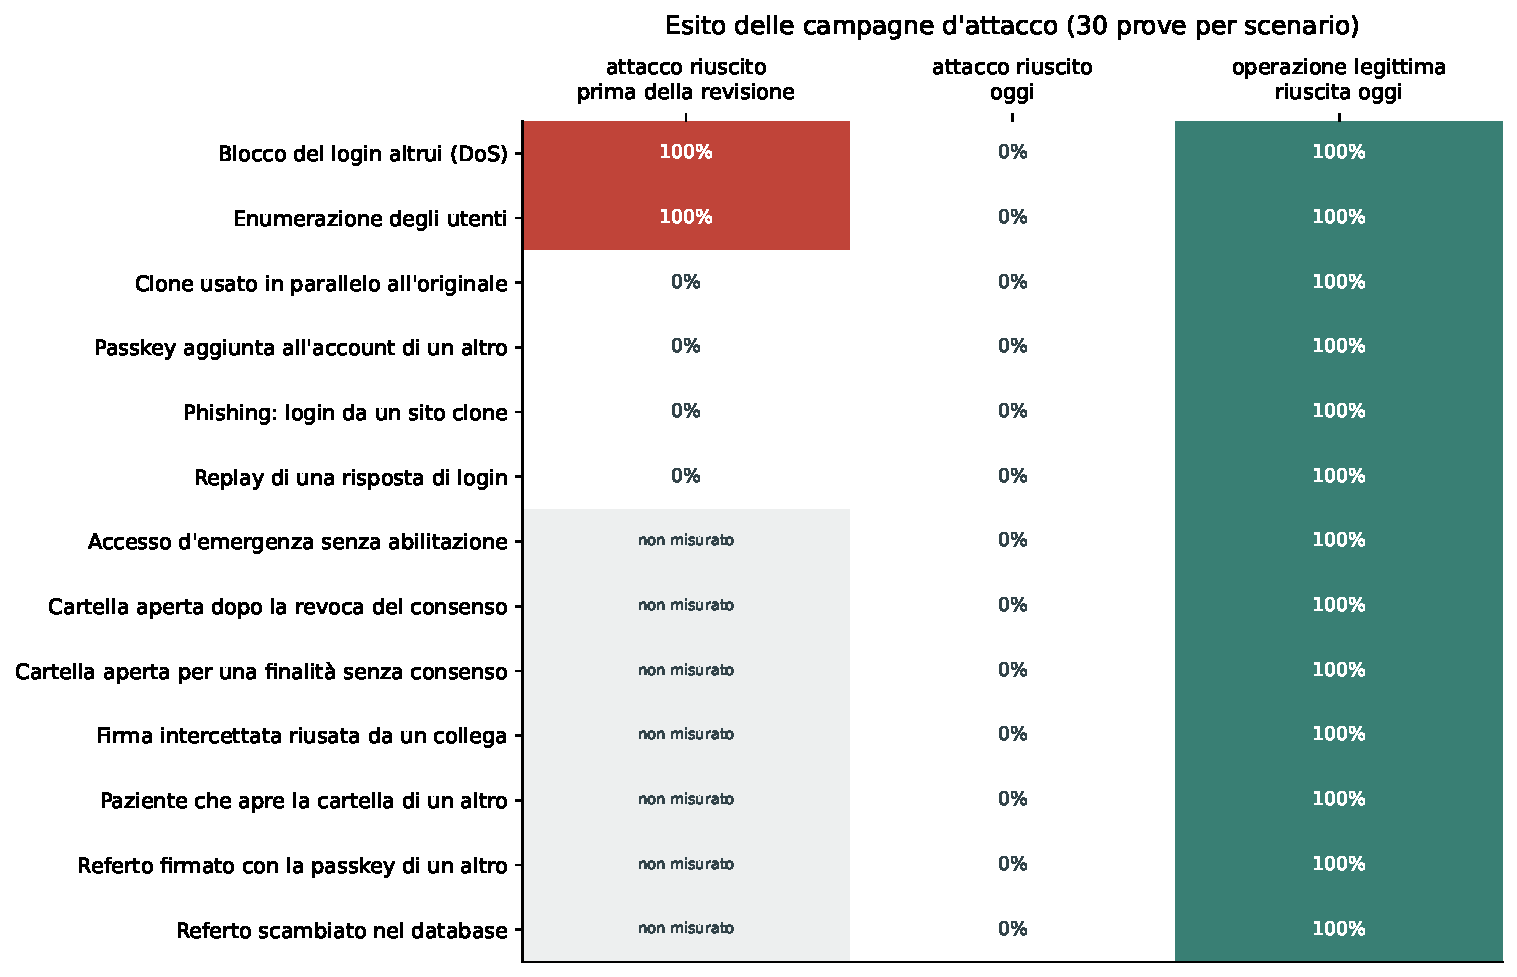
\includegraphics[width=\textwidth]{figure/attacchi_matrice.pdf}
\column{.4\textwidth}
\begin{itemize}
  \item ogni attacco ripetuto \alert{30 volte} contro il backend reale
  \item misurata anche l'operazione legittima: una difesa che blocca gli onesti non va bene
  \item \alert{nessun attacco riuscito}, tutte le operazioni legittime riuscite
\end{itemize}
\end{columns}
\end{frame}

% ---------------------------------------------------------------
\begin{frame}{Valutazione: costi}
\begin{columns}[c]
\column{.55\textwidth}
\centering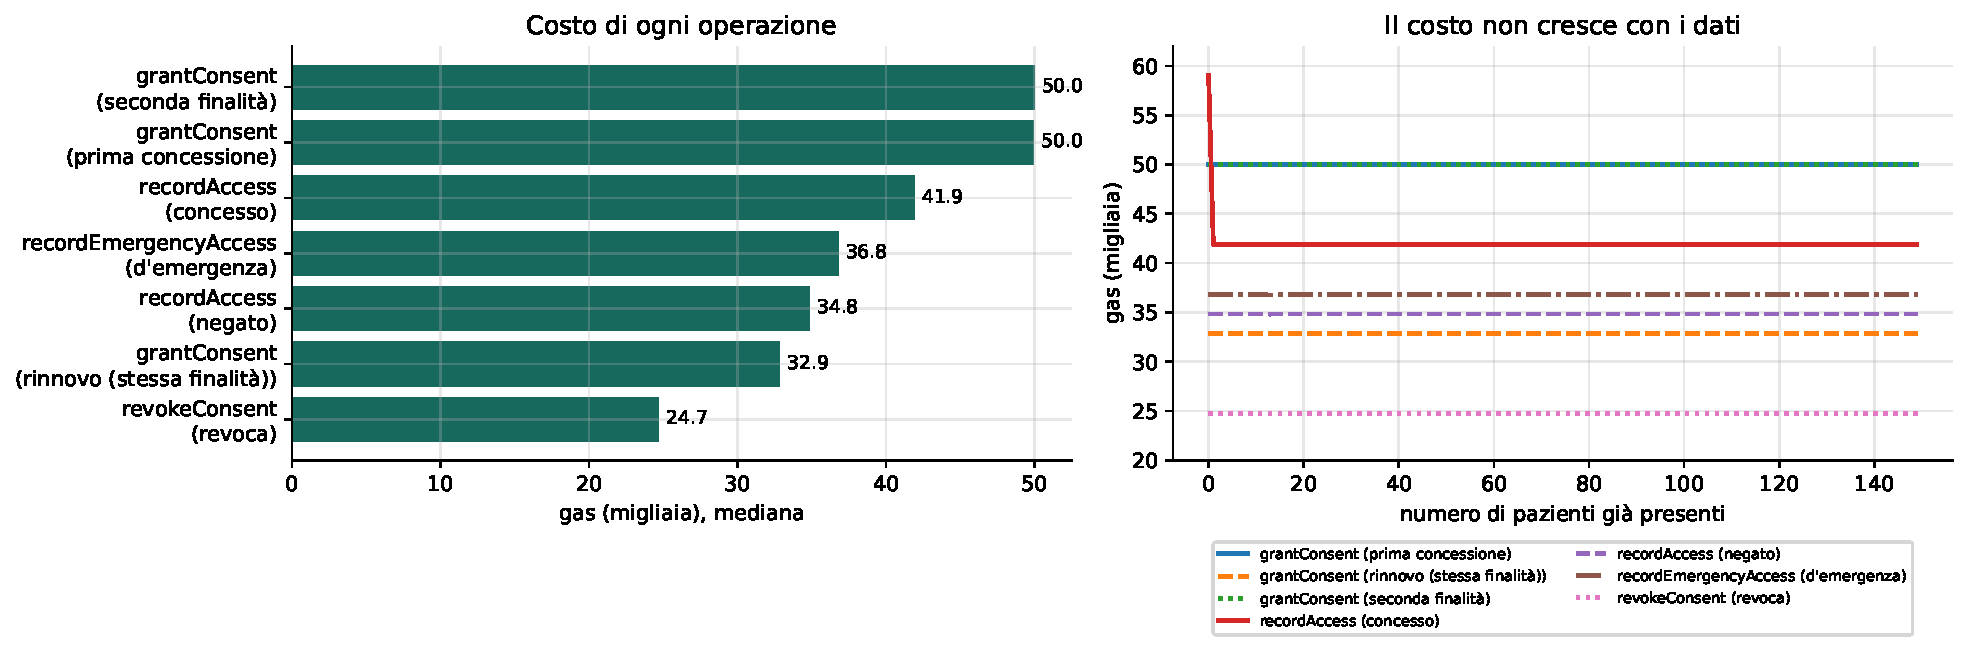
\includegraphics[width=\textwidth]{figure/gas_operazioni.pdf}
\column{.43\textwidth}
\begin{itemize}
  \item accesso registrato: \alert{\textasciitilde 42 mila} gas, costante al crescere dei registri
  \item cifrare un referto da 1 MiB: \alert{< 1 ms}
  \item verificare una firma ML-DSA: \textasciitilde 0,5 ms; il costo è nello spazio (firma da 2420 byte)
  \item Argon2id: \textasciitilde 70 ms per tentativo
\end{itemize}
\end{columns}
\end{frame}

% ---------------------------------------------------------------
\begin{frame}{Limiti e sviluppi futuri}
\begin{columns}[T]
\column{.48\textwidth}
\textbf{Limiti}
\begin{itemize}
  \item metadati collegabili su una catena pubblica
  \item un backend compromesso legge ciò che decifra
  \item chiavi in memoria a server acceso
\end{itemize}
\column{.48\textwidth}
\textbf{Sviluppi}
\begin{itemize}
  \item rete \emph{permissioned} (Hyperledger Fabric) con più organizzazioni
  \item abilitazione del medico con \alert{zk-SNARK} e pseudonimi per rapporto di cura
  \item chiavi in HSM o TEE, chiavi per paziente
  \item nuova verifica con la passkey per le operazioni sensibili
\end{itemize}
\end{columns}
\end{frame}

% ---------------------------------------------------------------
\begin{frame}{Conclusioni}
\begin{itemize}
  \item FIDO2 elimina le password e con esse il phishing.
  \item La blockchain toglie al backend la possibilità di decidere da solo chi legge una cartella e di nascondere un accesso.
  \item La cifratura e la separazione on-chain/off-chain impediscono che la trasparenza della catena diventi una fuga di dati.
\end{itemize}

\bigskip
\centering
\begin{tabular}{ccc}
\textbf{\Large 191} & \textbf{\Large 0} & \textbf{\Large 9/10} \\
test automatici & attacchi riusciti & requisiti funzionali\\
\end{tabular}

\bigskip
\small Codice: \texttt{github.com/Rcal97/sicurezza-dati-cartella-clinica-passwordless}
\end{frame}

\begin{frame}[standout]
Grazie
\end{frame}

\end{document}
